\chapter{Software Design Specification}
\label{chap:design}
\section{Product Architecture and Current Slice}
Figure~\ref{fig:planned-architecture} shows the six-module product design and marks later integrations. The current slice executes record loading, evidence presentation, profile/policy calculation and explanation recovery. Recorded scientific outputs enter through explicit artifact contracts; model training is not a page-load action.
\begin{figure}[htbp]\centering\resizebox{\linewidth}{!}{\begin{tikzpicture}[x=1mm,y=1mm,b/.style={draw,text width=39mm,minimum height=18mm,align=center,font=\sffamily\small},planned/.style={b,dashed,fill=gray!7},>=Stealth]
\node[b] (data) at (23,91){Data / sentiment\\Prices + news; social study};
\node[b] (engine) at (78,91){Predictive model\\XGBoost / calibration};
\node[b] (context) at (133,91){SHAP / context\\All values and definitions};
\node[b] (template) at (78,53){Current explanation\\Deterministic template};
\node[planned] (llm) at (133,53){Explanation layer (LLM)\\Planned: Mid-2};
\node[b] (profile) at (23,53){Investor profiling\\Trusted policy outcome};
\node[b] (guard) at (78,15){Explanation verifier\\Retain rejection / fallback};
\node[b] (ui) at (23,15){Interface / service\\Streamlit; service later};
\draw[->](data)--(engine);\draw[->](engine)--(context);
\draw[->](context.south west)--(template.north east);
\draw[->,dashed](context)--(llm);
\draw[->](template)--(guard);\draw[->,dashed](llm.south)--(133,15)--(guard.east);
\draw[->](profile)--(template);\draw[->,dashed](profile.north)--(23,68)--(133,68)--(llm.north);
\draw[->](profile.south)--(23,34)--(56,34)--(guard.north west);
\draw[->](guard)--(ui);
\end{tikzpicture}}
\caption{Six-module product architecture; dashed elements represent later integration.}\label{fig:planned-architecture}\end{figure}
\begin{figure}[htbp]\centering\resizebox{\linewidth}{!}{\begin{tikzpicture}[x=1mm,y=1mm,b/.style={draw,rounded corners,text width=63mm,minimum height=21mm,align=center,font=\sffamily\footnotesize},>=Stealth]
\node[b] (inputs) at (35,119){Versioned price/news snapshots\\Source, event and acquisition identity};\node[b] (features) at (35,83){Calendar/as-of alignment\\Causal indicators + FinBERT aggregates};\node[b] (science) at (35,47){Chronological model/calibration\\Available-label purge + controls};\node[b] (records) at (115,47){Validated decision records\\Probabilities, SHAP, values and hashes};\node[b] (services) at (115,83){Evidence, profile and claim services\\Confidence gate + checked recovery};\node[b] (view) at (115,119){Historical Streamlit workflow\\Current case/result identity};
\draw[->](inputs)--(features);\draw[->](features)--(science);\draw[->](science)--node[above,font=\scriptsize]{new identified outputs}(records);\draw[->](records)--(services);\draw[->](services)--(view);
\node[align=center,font=\sffamily\footnotesize] at (75,8){Offline scientific execution produces records.\\Interactive checking/profile logic uses them without retraining.};
\end{tikzpicture}}
\caption{Current data-to-record and record-to-interface pipeline.}\label{fig:pipeline}\end{figure}
\section{Components and Layers}
The interface calls context, profile and verification services. Scientific routines produce the versioned records read by those services. Local adapters and study readers use declared identities rather than silent substitution.
\begin{figure}[htbp]\centering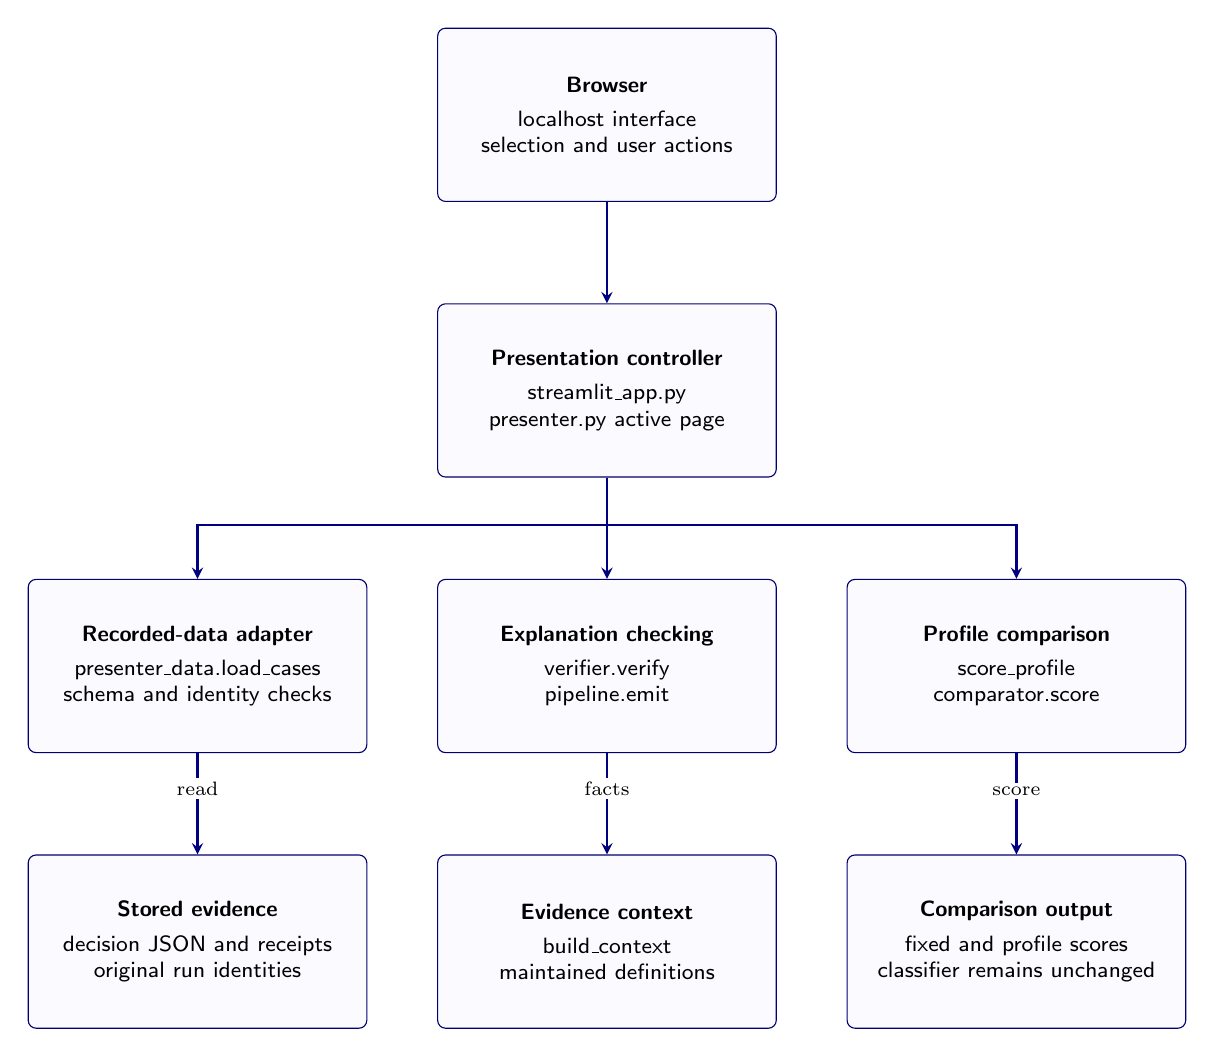
\begin{tikzpicture}[x=1mm,y=1mm,box/.style={draw=blue!45!black,fill=blue!2,rounded corners=1mm,align=center,text width=39mm,minimum height=22mm,inner sep=2mm,font=\sffamily\footnotesize},link/.style={->,>=stealth,draw=blue!50!black,thick}]
\node[box] (browser) at (75,140) {\textbf{Browser}\\[1mm]localhost interface\\selection and user actions};
\node[box] (presenter) at (75,105) {\textbf{Presentation controller}\\[1mm]streamlit\_app.py\\presenter.py active page};
\node[box] (loader) at (23,70) {\textbf{Recorded-data adapter}\\[1mm]presenter\_data.load\_cases\\schema and identity checks};
\node[box] (checking) at (75,70) {\textbf{Explanation checking}\\[1mm]verifier.verify\\pipeline.emit};
\node[box] (risk) at (127,70) {\textbf{Profile comparison}\\[1mm]score\_profile\\comparator.score};
\node[box] (artifacts) at (23,35) {\textbf{Stored evidence}\\[1mm]decision JSON and receipts\\original run identities};
\node[box] (context) at (75,35) {\textbf{Evidence context}\\[1mm]build\_context\\maintained definitions};
\node[box] (result) at (127,35) {\textbf{Comparison output}\\[1mm]fixed and profile scores\\classifier remains unchanged};
\draw[link] (browser.south) -- ++(0,-6) -| (presenter.north);
\draw[link] (presenter.south) -- ++(0,-6) -| (loader.north);
\draw[link] (presenter.south) -- ++(0,-6) -| (checking.north);
\draw[link] (presenter.south) -- ++(0,-6) -| (risk.north);
\draw[link] (loader.south) -- ++(0,-6) -| (artifacts.north) node[pos=.5,above,fill=white,inner sep=.5mm,font=\scriptsize]{read};
\draw[link] (checking.south) -- ++(0,-6) -| (context.north) node[pos=.5,above,fill=white,inner sep=.5mm,font=\scriptsize]{facts};
\draw[link] (risk.south) -- ++(0,-6) -| (result.north) node[pos=.5,above,fill=white,inner sep=.5mm,font=\scriptsize]{score};
\end{tikzpicture}
\caption{Implemented components and their interfaces.}\label{fig:components}\end{figure}
\begin{figure}[htbp]\centering\resizebox{\linewidth}{!}{\begin{tikzpicture}[x=1mm,y=1mm,b/.style={draw,text width=135mm,minimum height=23mm,align=center,font=\sffamily\footnotesize},>=Stealth]
\node[b] (ui) at (75,119){\textbf{Presentation}\\Overview / Decision / Evidence / Risk / Explanation / Studies};
\node[b] (app) at (75,81){\textbf{Application}\\Case loading, current-state ownership, confidence policy and emission};
\node[b] (domain) at (75,43){\textbf{Domain}\\Validated records, feature meanings, tolerance/capacity and claim checks};
\node[b] (files) at (75,5){\textbf{Artifacts / runtime}\\Versioned JSON traces, original models, study receipts and local session memory};
\draw[->](ui)--node[right,font=\scriptsize]{user action}(app);\draw[->](app)--node[right,font=\scriptsize]{validated contract}(domain);\draw[->](domain)--node[right,font=\scriptsize]{read / retain identity}(files);
\end{tikzpicture}}
\caption{Presentation, application, domain and artifact layers.}\label{fig:layers}\end{figure}
\section{Domain and Class Model}
The class model includes attributes and operations used by the code. Multiplicities distinguish a collection of records, a record's contributions and candidate/verification relationships. Profile evaluation is a dependency on a record, not a mutation of classifier probabilities.
\begin{figure}[p]\centering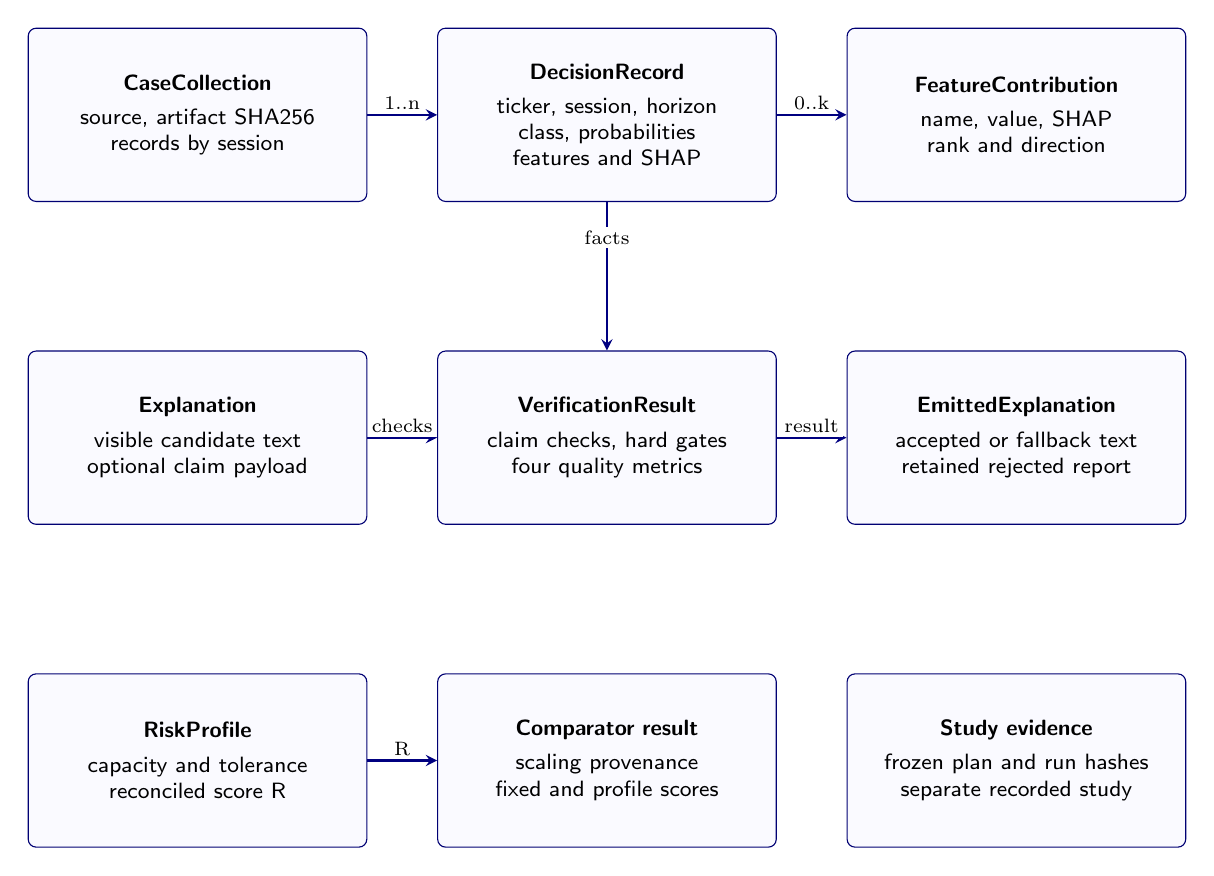
\begin{tikzpicture}[x=1mm,y=1mm,box/.style={draw=blue!45!black,fill=blue!2,rounded corners=1mm,align=center,text width=39mm,minimum height=22mm,inner sep=2mm,font=\sffamily\footnotesize},link/.style={->,>=stealth,draw=blue!50!black,thick}]
\node[box] (collection) at (23,100) {\textbf{CaseCollection}\\[1mm]source, artifact SHA256\\records by session};
\node[box] (record) at (75,100) {\textbf{DecisionRecord}\\[1mm]ticker, session, horizon\\class, probabilities\\features and SHAP};
\node[box] (contrib) at (127,100) {\textbf{FeatureContribution}\\[1mm]name, value, SHAP\\rank and direction};
\node[box] (explanation) at (23,59) {\textbf{Explanation}\\[1mm]visible candidate text\\optional claim payload};
\node[box] (verification) at (75,59) {\textbf{VerificationResult}\\[1mm]claim checks, hard gates\\four quality metrics};
\node[box] (emission) at (127,59) {\textbf{EmittedExplanation}\\[1mm]accepted or fallback text\\retained rejected report};
\node[box] (profile) at (23,18) {\textbf{RiskProfile}\\[1mm]capacity and tolerance\\reconciled score R};
\node[box] (comparison) at (75,18) {\textbf{Comparator result}\\[1mm]scaling provenance\\fixed and profile scores};
\node[box] (study) at (127,18) {\textbf{Study evidence}\\[1mm]frozen plan and run hashes\\separate recorded study};
\draw[link] (collection.east) -- (record.west) node[pos=.5,above,fill=white,inner sep=.5mm,font=\scriptsize]{1..n};
\draw[link] (record.east) -- (contrib.west) node[pos=.5,above,fill=white,inner sep=.5mm,font=\scriptsize]{0..k};
\draw[link] (record.south) -- ++(0,-6) -| (verification.north) node[pos=.5,above,fill=white,inner sep=.5mm,font=\scriptsize]{facts};
\draw[link] (explanation.east) -- (verification.west) node[pos=.5,above,fill=white,inner sep=.5mm,font=\scriptsize]{checks};
\draw[link] (verification.east) -- (emission.west) node[pos=.5,above,fill=white,inner sep=.5mm,font=\scriptsize]{result};
\draw[link] (profile.east) -- (comparison.west) node[pos=.5,above,fill=white,inner sep=.5mm,font=\scriptsize]{R};
\end{tikzpicture}
\caption{Implementation class model with attributes, operations and multiplicities.}\label{fig:classes}\end{figure}
\section{Data Flow and File Schema}
The schema identifies experiment and composite case identities, keyed feature maps, candidate digests and result ownership. These are JSON/file/session contracts, not a claimed SQL database. Relationship labels and cardinalities express how the actual loader and checker bind their data.
\begin{figure}[htbp]\centering\resizebox{\linewidth}{!}{\begin{tikzpicture}[x=1mm,y=1mm,b/.style={draw,rounded corners,text width=49mm,minimum height=24mm,align=center,font=\sffamily\footnotesize},store/.style={draw,double,text width=49mm,minimum height=19mm,align=center,font=\sffamily\footnotesize},>=Stealth]
\node[b] (user) at (75,146){User: selection, answers and candidate};\node[b] (loader) at (32,106){P1: load/validate\\Case + source identity};\node[b] (profile) at (118,106){P2: score profile/policy\\Capacity, tolerance, allowance};
\node[b] (check) at (32,61){P3: verify claims\\Candidate and source independently};\node[b] (emit) at (118,61){P4: emit current result\\Accepted, fallback or error};
\node[store] (files) at (32,13){D1: recorded artifacts / receipts};\node[store] (state) at (118,13){D2: session profile / result identity};
\draw[->](user.south)-|node[pos=.35,above,font=\scriptsize]{case/text}(loader.north);\draw[->](user.south)-|node[pos=.35,above,font=\scriptsize]{18 answers}(profile.north);
\draw[->](files.west)--(-5,13)--node[left,font=\scriptsize]{record}(-5,106)--(loader.west);\draw[->](loader)--(check);\draw[->](check)--node[above,font=\scriptsize]{verdict}(emit);\draw[->](profile)--node[right,font=\scriptsize]{policy result}(emit);\draw[->](emit)--(state);
\draw[->](emit.east)--(153,61)--(153,146)--node[above,font=\scriptsize]{current display}(user.east);
\end{tikzpicture}}
\caption{Data flow through the current checking and policy path.}\label{fig:dataflow}\end{figure}
\begin{figure}[p]\centering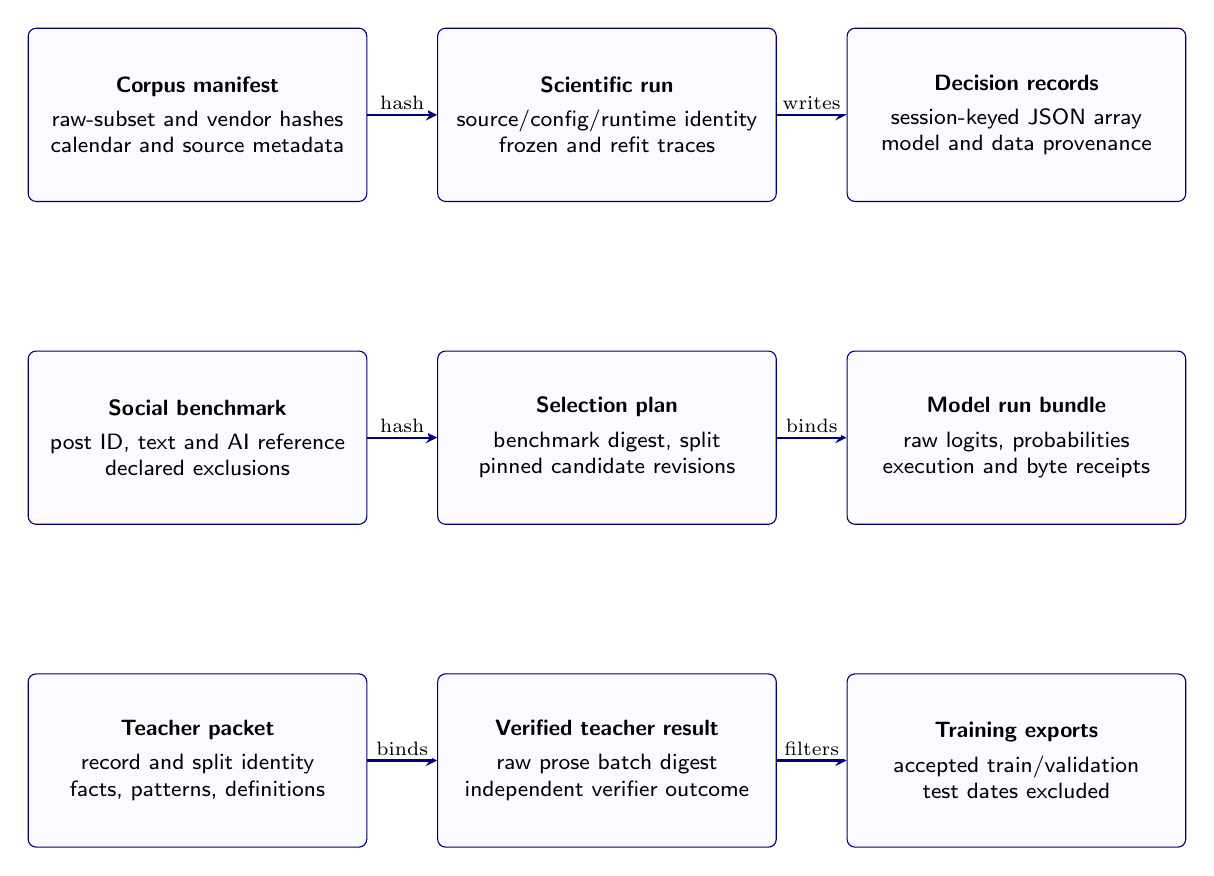
\begin{tikzpicture}[x=1mm,y=1mm,box/.style={draw=blue!45!black,fill=blue!2,rounded corners=1mm,align=center,text width=39mm,minimum height=22mm,inner sep=2mm,font=\sffamily\footnotesize},link/.style={->,>=stealth,draw=blue!50!black,thick}]
\node[box] (manifest) at (23,105) {\textbf{Corpus manifest}\\[1mm]raw-subset and vendor hashes\\calendar and source metadata};
\node[box] (run) at (75,105) {\textbf{Scientific run}\\[1mm]source/config/runtime identity\\frozen and refit traces};
\node[box] (records) at (127,105) {\textbf{Decision records}\\[1mm]session-keyed JSON array\\model and data provenance};
\node[box] (benchmark) at (23,64) {\textbf{Social benchmark}\\[1mm]post ID, text and AI reference\\declared exclusions};
\node[box] (plan) at (75,64) {\textbf{Selection plan}\\[1mm]benchmark digest, split\\pinned candidate revisions};
\node[box] (bundle) at (127,64) {\textbf{Model run bundle}\\[1mm]raw logits, probabilities\\execution and byte receipts};
\node[box] (packet) at (23,23) {\textbf{Teacher packet}\\[1mm]record and split identity\\facts, patterns, definitions};
\node[box] (teacher) at (75,23) {\textbf{Verified teacher result}\\[1mm]raw prose batch digest\\independent verifier outcome};
\node[box] (exports) at (127,23) {\textbf{Training exports}\\[1mm]accepted train/validation\\test dates excluded};
\draw[link] (manifest.east) -- (run.west) node[pos=.5,above,fill=white,inner sep=.5mm,font=\scriptsize]{hash};
\draw[link] (run.east) -- (records.west) node[pos=.5,above,fill=white,inner sep=.5mm,font=\scriptsize]{writes};
\draw[link] (benchmark.east) -- (plan.west) node[pos=.5,above,fill=white,inner sep=.5mm,font=\scriptsize]{hash};
\draw[link] (plan.east) -- (bundle.west) node[pos=.5,above,fill=white,inner sep=.5mm,font=\scriptsize]{binds};
\draw[link] (packet.east) -- (teacher.west) node[pos=.5,above,fill=white,inner sep=.5mm,font=\scriptsize]{binds};
\draw[link] (teacher.east) -- (exports.west) node[pos=.5,above,fill=white,inner sep=.5mm,font=\scriptsize]{filters};
\end{tikzpicture}
\caption{Artifact/session schema with keys and relationship cardinalities.}\label{fig:schema}\end{figure}
\section{Behavioral Design}
The sequence starts with the actual Check explanation click and uses alternative fragments for acceptance and recovery. The activity includes invalid input and fallback-verification failure. The state model includes initialization, stale results, errors and session termination.
\begin{figure}[p]\centering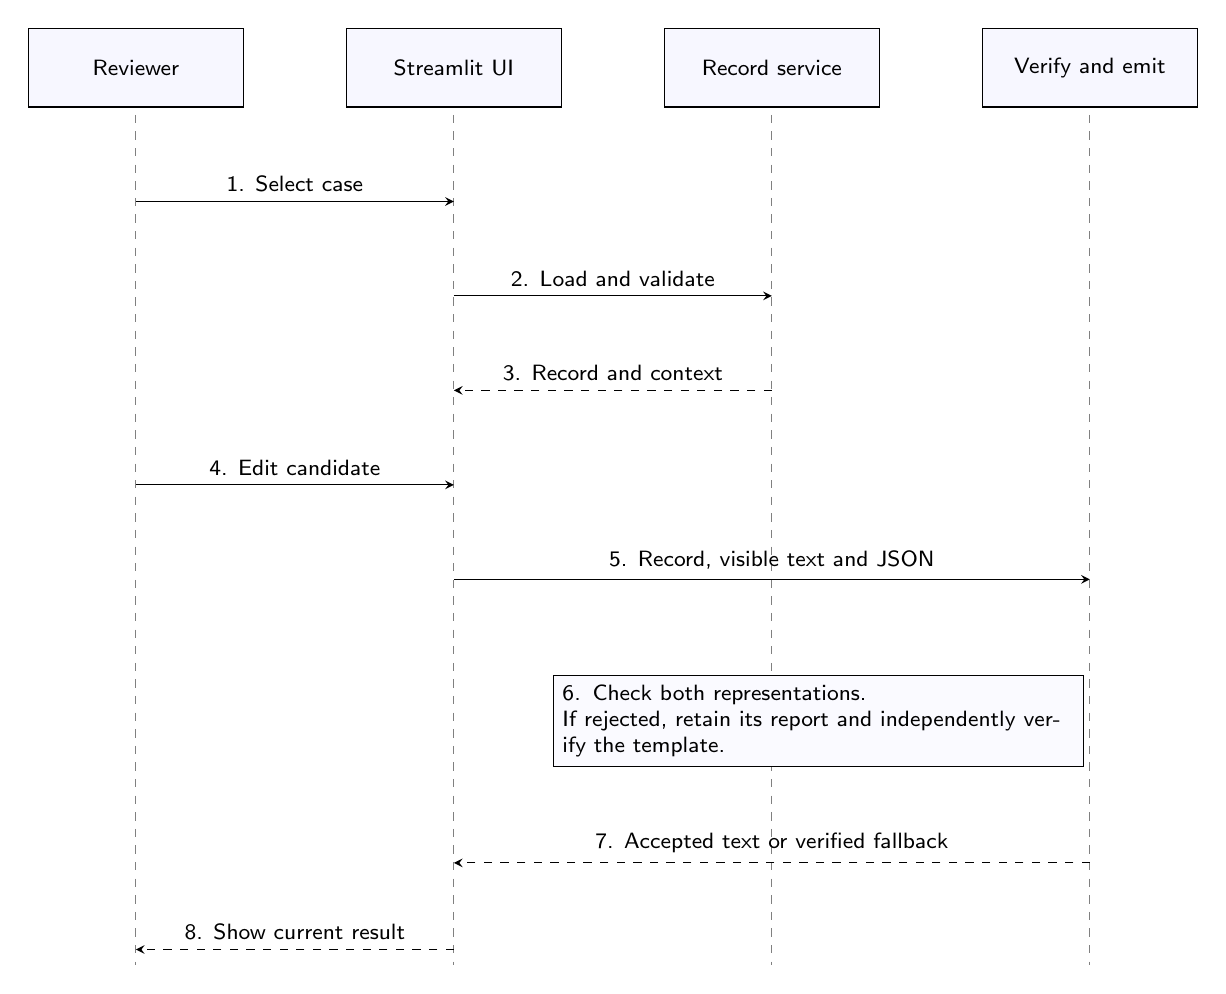
\begin{tikzpicture}[x=.985mm,y=1mm,font=\sffamily\footnotesize,>=stealth]
\foreach \x/\n in {12/Reviewer,53/Streamlit UI,94/Record service,135/Verify and emit}{
\node[draw,fill=blue!3,text width=25mm,align=center,minimum height=10mm] at (\x,122){\n};
\draw[dashed,gray] (\x,116)--(\x,8);}
\draw[->] (12,105)--node[above]{1. Select case}(53,105);
\draw[->] (53,93)--node[above]{2. Load and validate}(94,93);
\draw[->,dashed] (94,81)--node[above]{3. Record and context}(53,81);
\draw[->] (12,69)--node[above]{4. Edit candidate}(53,69);
\draw[->] (53,57)--node[above]{5. Record, visible text and JSON}(135,57);
\node[align=left,text width=65mm,fill=blue!2,draw] at (100,39){6. Check both representations.\\If rejected, retain its report and independently verify the template.};
\draw[->,dashed] (135,21)--node[above]{7. Accepted text or verified fallback}(53,21);
\draw[->,dashed] (53,10)--node[above]{8. Show current result}(12,10);
\end{tikzpicture}
\caption{Explanation-check sequence with explicit user trigger and alternative outcomes.}\label{fig:sequence}\end{figure}
\begin{figure}[p]\centering\resizebox{\linewidth}{!}{\begin{tikzpicture}[x=1mm,y=1mm,b/.style={draw,rounded corners,text width=48mm,minimum height=15mm,align=center,font=\sffamily\footnotesize},d/.style={draw,diamond,aspect=2.5,align=center,font=\sffamily\scriptsize,inner sep=1mm},>=Stealth]
\node[circle,fill,minimum size=3mm,inner sep=0] (start) at (75,192){};
\node[b] (load) at (75,175){Load and validate selected record};\node[d] (valid) at (75,151){Valid?};
\node[b] (candidate) at (75,126){Read current text/payload; verify independently};\node[d] (pass) at (75,101){Candidate passes?};
\node[b] (accept) at (28,76){Emit candidate and accepted report};\node[b] (fallback) at (122,76){Retain rejection; render fallback};
\node[d] (fallbackpass) at (122,46){Fallback passes?};\node[b] (emit) at (76,18){Emit checked replacement};\node[b] (error) at (20,18){Show error; no verified output};
\node[circle,draw,double,fill=black,minimum size=4mm,inner sep=0] (end) at (75,-11){};
\draw[->](start)--(load);\draw[->](load)--(valid);\draw[->](valid)--node[right]{yes}(candidate);\draw[->](candidate)--(pass);
\draw[->](valid.west)--node[above]{no}(-15,151)--(-15,18)--(error.west);
\draw[->](pass.west)-|node[pos=.25,above]{yes}(accept.north);\draw[->](pass.east)-|node[pos=.25,above]{no}(fallback.north);
\draw[->](fallback)--(fallbackpass);\draw[->](fallbackpass.south)|-node[pos=.25,above]{yes}(emit.east);
\draw[->](fallbackpass.east)--node[above]{no}(154,46)--(154,0)--(20,0)--(error.south);
\draw[->](accept.south)--(28,55)--(-30,55)--(-30,-11)--(end.west);
\draw[->](emit.south)--(end.north);\draw[->](error.south)|-(end.west);
\end{tikzpicture}}
\caption{Checking activity, including verified fallback and error termination.}\label{fig:activity}\end{figure}
\begin{figure}[p]\centering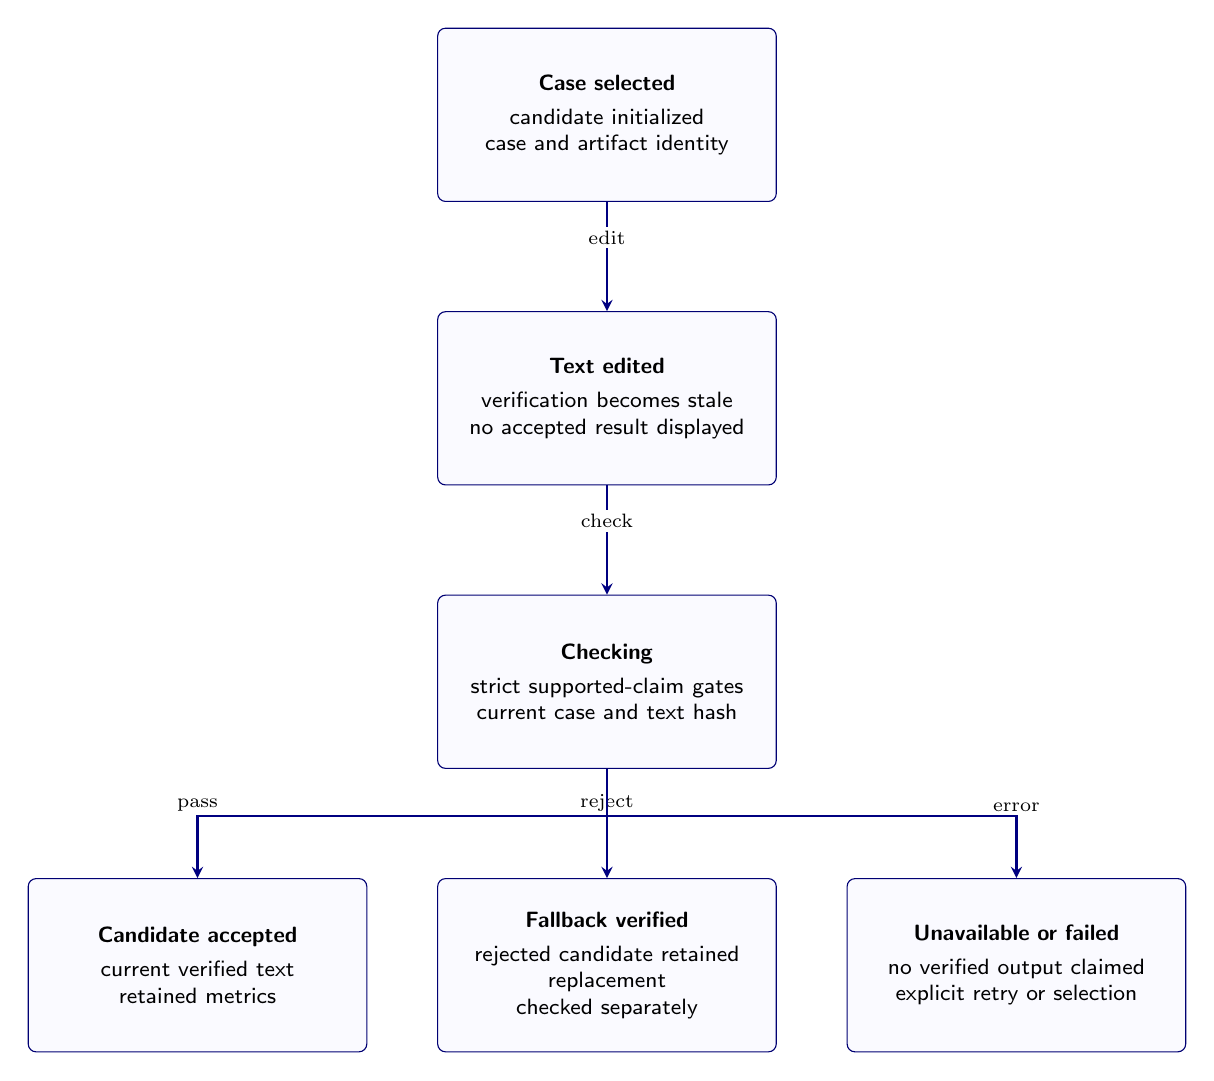
\begin{tikzpicture}[x=1mm,y=1mm,box/.style={draw=blue!45!black,fill=blue!2,rounded corners=1mm,align=center,text width=39mm,minimum height=22mm,inner sep=2mm,font=\sffamily\footnotesize},link/.style={->,>=stealth,draw=blue!50!black,thick}]
\node[box] (selected) at (75,135) {\textbf{Case selected}\\[1mm]candidate initialized\\case and artifact identity};
\node[box] (edited) at (75,99) {\textbf{Text edited}\\[1mm]verification becomes stale\\no accepted result displayed};
\node[box] (checking) at (75,63) {\textbf{Checking}\\[1mm]strict supported-claim gates\\current case and text hash};
\node[box] (accepted) at (23,27) {\textbf{Candidate accepted}\\[1mm]current verified text\\retained metrics};
\node[box] (fallback) at (75,27) {\textbf{Fallback verified}\\[1mm]rejected candidate retained\\replacement checked separately};
\node[box] (error) at (127,27) {\textbf{Unavailable or failed}\\[1mm]no verified output claimed\\explicit retry or selection};
\draw[link] (selected.south) -- ++(0,-6) -| (edited.north) node[pos=.5,above,fill=white,inner sep=.5mm,font=\scriptsize]{edit};
\draw[link] (edited.south) -- ++(0,-6) -| (checking.north) node[pos=.5,above,fill=white,inner sep=.5mm,font=\scriptsize]{check};
\draw[link] (checking.south) -- ++(0,-6) -| (accepted.north) node[pos=.5,above,fill=white,inner sep=.5mm,font=\scriptsize]{pass};
\draw[link] (checking.south) -- ++(0,-6) -| (fallback.north) node[pos=.5,above,fill=white,inner sep=.5mm,font=\scriptsize]{reject};
\draw[link] (checking.south) -- ++(0,-6) -| (error.north) node[pos=.5,above,fill=white,inner sep=.5mm,font=\scriptsize]{error};
\end{tikzpicture}
\caption{Case/candidate verification state transitions.}\label{fig:state}\end{figure}
\section{Deployment and Design Evolution}
The localhost browser communicates with Streamlit. Core modules read registered artifacts and retain profile/candidate state in memory. CI produces downloadable review artifacts; it does not host the application. The revised deployment model includes the core-to-artifact link.
\begin{figure}[htbp]\centering\resizebox{\linewidth}{!}{\begin{tikzpicture}[x=1mm,y=1mm,b/.style={draw,rounded corners,text width=62mm,minimum height=27mm,align=center,font=\sffamily\footnotesize},>=Stealth]
\node[b] (browser) at (75,146){\textless\textless device\textgreater\textgreater\\Browser on project/groupmate laptop};
\node[b] (server) at (75,96){\textless\textless execution environment\textgreater\textgreater\\Python 3.11 / Streamlit, loopback 8507\\Presenter + core context/profile/verifier};
\node[b] (files) at (33,40){\textless\textless artifact\textgreater\textgreater\\Recorded cases, traces and study receipts};\node[b] (memory) at (117,40){\textless\textless session state\textgreater\textgreater\\Profile, candidate and current result};
\draw[->](browser)--node[right,font=\scriptsize]{HTTP / WebSocket}(server);
\draw[->](server.south)-|node[pos=.25,above,font=\scriptsize]{core reads}(files.north);\draw[->](server.south)-|node[pos=.25,above,font=\scriptsize]{local state}(memory.north);
\node[draw,dashed,text width=137mm,align=center,font=\sffamily\footnotesize,inner sep=3mm] (ci) at (75,-5){GitHub Actions: Windows/Ubuntu checks $\rightarrow$ verified downloadable source/PDF artifact. Production hosting and trained-student serving are later deployment targets.};
\draw[->,dashed](ci.north west)--node[left,font=\scriptsize]{clone / extract}(files.south west);
\end{tikzpicture}}
\caption{Current localhost deployment and artifact-delivery boundary.}\label{fig:deployment}\end{figure}
The proposal's broad product design is retained, while the implemented slice now has complete evidence, independent prose/JSON checks, a full scored profile and uncertainty gating. The prior risk-dependent sentiment blend and isotonic outputs remain historical comparisons. Broader conversation, social divergence and production service work are explicitly scheduled.
\section{Algorithms and Contracts}
Record validation precedes display. Checking retains candidate errors, constructs fallback and verifies it independently. Temperature fitting admits only earlier-matured calibration labels. Profile scoring validates every answer, calculates weighted capacity/caps and published item totals, reconciles restrictive limits and evaluates confidence without changing direction. Each boundary carries identity and failure conditions used by its tests.
